\documentclass[12pt,letterpaper]{article}
\usepackage{graphicx,textcomp}
\usepackage{natbib}
\usepackage{setspace}
\usepackage{fullpage}
\usepackage{color}
\usepackage[reqno]{amsmath}
\usepackage{amsthm}
\usepackage{fancyvrb}
\usepackage{amssymb,enumerate}
\usepackage[all]{xy}
\usepackage{endnotes}
\usepackage{lscape}
\usepackage{float}
\usepackage{hyperref}
\usepackage[compact]{titlesec}
\usepackage{dcolumn}
\usepackage{tikz}
\usetikzlibrary{arrows}
\usepackage{multirow}
\usepackage{xcolor}
\usepackage{url}
\usepackage{listings}

\newtheorem{com}{Comment}
\newtheorem{lem}{Lemma}
\newtheorem{prop}{Proposition}
\newtheorem{thm}{Theorem}
\newtheorem{defn}{Definition}
\newtheorem{cor}{Corollary}
\newtheorem{obs}{Observation}
\newtheorem{hyp}{Hypothesis}

\newcolumntype{.}{D{.}{.}{-1}}
\newcolumntype{d}[1]{D{.}{.}{#1}}
\definecolor{light-gray}{gray}{0.65}
\definecolor{codegreen}{rgb}{0,0.6,0}
\definecolor{codegray}{rgb}{0.5,0.5,0.5}
\definecolor{codepurple}{rgb}{0.58,0,0.82}
\definecolor{backcolour}{rgb}{0.95,0.95,0.92}

\lstdefinestyle{mystyle}{
	backgroundcolor=\color{backcolour},
	commentstyle=\color{codegreen},
	keywordstyle=\color{magenta},
	numberstyle=\tiny\color{codegray},
	stringstyle=\color{codepurple},
	basicstyle=\footnotesize,
	breakatwhitespace=false,
	breaklines=true,
	captionpos=b,
	keepspaces=true,
	numbers=left,
	numbersep=5pt,
	showspaces=false,
	showstringspaces=false,
	showtabs=false,
	tabsize=2
}
\lstset{style=mystyle}

\newcommand{\Sref}[1]{Section~\ref{#1}}


\setstretch{1.2}
\usepackage{parskip}


\titlespacing*{\section}{0pt}{1.2\baselineskip}{0.8\baselineskip}
\titlespacing*{\subsection}{0pt}{1\baselineskip}{0.6\baselineskip}

\title{Problem Set 2}
\date{\today}
\author{Hanyu Li(Student ID:25346841)}

\begin{document}
	\maketitle
	
	\section*{Instructions}
	\begin{itemize}
		\item Please show your work! You may lose points by simply writing in the answer. If the problem requires you to execute commands in \texttt{R}, please include the code you used to get your answers. Please also include the \texttt{.R} file that contains your code. If you are not sure if work needs to be shown for a particular problem, please ask.
		\item Your homework should be submitted electronically on GitHub.
		\item This problem set is due before 23:59 on Thursday October 23, 2025. No late assignments will be accepted.
	\end{itemize}
	
	\section*{Question 1: Political Science}
	The following table was created using the data from a study run in a major Latin American city.\footnote{Fried, Lagunes, and Venkataramani (2010). `Corruption and Inequality at the Crossroad: A Multimethod Study of Bribery and Discrimination in Latin America. \textit{Latin American Research Review}. 45 (1): 76-97.} 
	As part of the experimental treatment in the study, one employee of the research team was chosen to make illegal left turns across traffic to draw the attention of the police officers on shift. Two employee drivers were upper class, two were lower class drivers, and the identity of the driver was randomly assigned per encounter. The researchers were interested in whether officers were more or less likely to solicit a bribe from drivers depending on their class (officers use phrases like, "We can solve this the easy way" to draw a bribe). The table below shows the resulting data.
	
	\begin{table}[h!]
		\centering
		\begin{tabular}{l | c c c }
			& Not Stopped & Bribe requested & Stopped/given warning \\ \\[-1.8ex] \hline \\[-1.8ex]
			Upper class & 14 & 6 & 7 \\
			Lower class & 7 & 7 & 1 \\
			\hline
		\end{tabular}
	\end{table}
	
	\begin{enumerate}
		\item [(a)] Calculate the $\chi^2$ test statistic by hand/manually (even better if you can do "by hand" in \texttt{R}).\\
		This study examines the statistical independence between two categorical variables: the social class of employee drivers and whether police officers solicit bribes for traffic violations.
		
		Thus, the null hypothesis ($H_0$)is:
		Officers' bribery solicitation and employee drivers' social class are statistically independent.
		
		The alternative hypothesis ($H_1$) is:
		Officers' bribery solicitation and employee drivers' social class are statistically dependent.
		
		Based on the hypotheses, the expected frequency for each cell in the table is first calculated using the formula:
		\[
		E_{ij} = \frac{(\text{Row total}) \times (\text{Column total})}{\text{Grand total}}
		\]
		
		Next, using the observed and expected frequencies, the chi-square statistic $\chi^2$ is computed as:
		\[
		\chi^2 = \sum \frac{(f_o - f_e)^2}{f_e}
		\]
		
		The R code lines are as below:
		\lstinputlisting[language=R, firstline=2, lastline=22]{PS02_HL.R}
		
		The manual calculation in R yields a chi-square value of 3.4125, indicating some discrepancy between the observed and expected frequency distributions. Further testing is required to draw a final conclusion.
		
		\item [(b)] Now calculate the p-value from the test statistic you just created (in \texttt{R}).\footnote{Remember frequency should be $>$ 5 for all cells, but let's calculate the p-value here anyway.} What do you conclude if $\alpha = 0.1$?
		
		To calculate the p-value, the degrees of freedom for this contingency table must first be determined using the formula:
		\[
		df = (\text{rows} - 1) \times (\text{columns} - 1)
		\]
		
		Subsequently, the p-value is computed using the pchisq() function in R.
		
		The R code lines are as below:
		\lstinputlisting[language=R, firstline=24, lastline=26]{PS02_HL.R}
		
		The calculated p-value is 0.1502306. At a significance level of 0.1, this indicates that if the null hypothesis were true, the probability of observing the obtained frequency distribution would be approximately 15\%. Since this is greater than a significance level of 10\%, we do not have sufficient evidence to reject the null hypothesis. Thus, it can be concluded that the social class of employee drivers and bribery solicitation by police officers are statistically independent.
		
		\item [(c)] Calculate the standardized residuals for each cell and put them in the table below.
		
		\begin{table}[H]
			\centering
			\begin{tabular}{l | c c c }
				& Not Stopped & Bribe requested & Stopped/given warning \\ \\[-1.8ex] \hline \\[-1.8ex]
				Upper class &0.3220306 & -1.516426 & 1.649103 \\ \\ 
				Lower class & -0.2740361 & 1.929528 & -1.523026 \\
			\end{tabular}
		\end{table}
		
		\item [(d)] How might the standardized residuals help you interpret the results?
		
		The standardized residuals table shows that the absolute value of every residual is below 2, indicating no substantial discrepancies between any observed and expected frequencies. This finding further corroborates the modest chi-square statistic from Q1(a) and supports the decision in Q1(b) to retain the null hypothesis of statistical independence between a driver's social class and bribery solicitation by police officers.
		
	\end{enumerate}
	
	\section*{Question 2: Economics}
	Chattopadhyay and Duflo were interested in whether women promote different policies than men.\footnote{Chattopadhyay and Duflo. (2004). `Women as Policy Makers: Evidence from a Randomized Policy Experiment in India. \textit{Econometrica}. 72 (5), 1409-1443.} Answering this question with observational data is pretty difficult due to potential confounding problems (e.g. the districts that choose female politicians are likely to systematically differ in other aspects too). Hence, they exploit a randomized policy experiment in India, where since the mid-1990s, $\frac{1}{3}$ of village council heads have been randomly reserved for women. A subset of the data from West Bengal can be found at the following link: \url{https://raw.githubusercontent.com/kosukeimai/qss/master/PREDICTION/women.csv}
	
	Each observation in the data set represents a village and there are two villages associated with one GP (i.e. a level of government is called "GP"). Figure~\ref{fig:women_desc} below shows the names and descriptions of the variables in the dataset. The authors hypothesize that female politicians are more likely to support policies female voters want. Researchers found that more women complain about the quality of drinking water than men. You need to estimate the effect of the reservation policy on the number of new or repaired drinking water facilities in the villages.
	
	\begin{figure}[H]
		\centering
		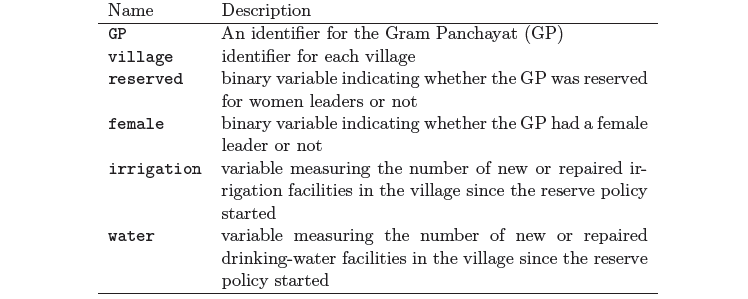
\includegraphics[width=1.1\textwidth]{women_desc.png}
		\caption{\footnotesize{Names and description of variables from Chattopadhyay and Duflo (2004).}}
		\label{fig:women_desc}
	\end{figure}
	
	\begin{enumerate}
		\item [(a)] State a null and alternative (two-tailed) hypothesis.
		
		To estimate the effect of female leaders' reservations in Gram Panchayats (GP) on the number of drinking water facilities, while controlling for other confounding factors, we use a simple linear regression model for hypothesis testing and prediction. The regression model is specified as:
		\[
		Y_i = \alpha + \beta X_i + \epsilon_i
		\]
		where $Y_i$ denotes the number of new or repaired drinking water facilities in village $i$, $X_i$ is a binary variable indicating whether the GP leadership is reserved for a female leader, $\alpha$ is the intercept, $\beta$ measures the effect of female leadership reservation, and $\epsilon_i$ is the error term.
		
		The hypotheses are formulated as follows:
		\[
		\text{Null hypothesis: } H_0: \beta = 0
		\]
		which states that female leaders' reservations in GP ($X$) have no effect on the number of drinking water facilities ($Y$), and
		\[
		\text{Alternative hypothesis: } H_1: \beta \neq 0
		\]
		which states that female leaders' reservations in GP ($X$) do have an effect on the number of drinking water facilities ($Y$).
		
		\item [(b)] Run a bivariate regression to test this hypothesis in \texttt{R} (include your code!).
		
		After importing the data, the structure and distribution were examined, and basic data cleaning was performed. \\
		
		\begin{verbatim}
			GP         village           reserved       female         irrigation    
			Min.   :  1   Min.   :1.0   NotReserved:214   Min.   :0.0000   Min.   : 0.000  
			1st Qu.: 41   1st Qu.:1.0   Reserved   :108   1st Qu.:0.0000   1st Qu.: 0.000  
			Median : 81   Median :1.5                     Median :0.0000   Median : 0.000  
			Mean   : 81   Mean   :1.5                     Mean   :0.3851   Mean   : 3.264  
			3rd Qu.:121   3rd Qu.:2.0                     3rd Qu.:1.0000   3rd Qu.: 2.000  
			Max.   :161   Max.   :2.0                     Max.   :1.0000   Max.   :90.000  
			water       
			Min.   :  0.00  
			1st Qu.:  3.00  
			Median :  9.00  
			Mean   : 17.84  
			3rd Qu.: 20.00  
			Max.   :340.00  
		\end{verbatim}
		
		A linear regression model was then fitted. The code and regression results are as follows:
		
		\lstinputlisting[language=R, firstline=32, lastline=44]{PS02_HL.R}
		
		\begin{table}[!htbp]
			\centering
			\caption{Regression Results}
			\begin{tabular}{@{\extracolsep{5pt}}lc}
				\\[-1.8ex]\hline \hline \\[-1.8ex]
				& \multicolumn{1}{c}{\textit{Dependent variable:}} \\
				\cline{2-2} \\[-1.8ex]
				& Number of Drinking Water Facilities \\
				\hline \\[-1.8ex]
				Intercept & 9.252$^{**}$ \\
				& (3.948) \\
				& \\
				Reserved (Female) & 14.738$^{***}$ \\
				& (2.286) \\
				& \\
				\hline \\[-1.8ex]
				Observations & 322 \\
				R$^{2}$ & 0.017 \\
				Adjusted R$^{2}$ & 0.014 \\
				Residual Std. Error & 33.446 (df = 320) \\
				F Statistic & 5.493$^{**}$ (df = 1; 320) \\
				\hline \hline \\[-1.8ex]
				\textit{Note:} & \multicolumn{1}{r}{$^{*}$p$<$0.1; $^{**}$p$<$0.05; $^{***}$p$<$0.01} \\
			\end{tabular}
		\end{table}
		
		The intercept (\(\alpha = 14.738\)) indicates that when the GP leadership is not reserved for a female leader, the average number of new or repaired drinking water facilities is about 14.7.
		
		The p-value for the model is 0.0197. At a significance level of 0.05, this is less than 0.05, providing evidence to support the alternative hypothesis: female leaders' reservations in GP have a significant effect on the number of drinking water facilities. The positive coefficient indicates that the reservation of female leadership increases the number of facilities built or repaired in the villages.
		
		However, the adjusted \(R\)-squared is only 0.014, very close to zero, indicating that the model does not fit the data well. The reservation of female leadership explains only a small part of the variation in the number of new or repaired drinking water facilities.
		
		\item [(c)] Interpret the coefficient estimate for reservation policy.
		
		The coefficient estimate of 9.252 in the model
		\[
		Y_i = 14.738 + 9.252 X_i
		\]
		
		can be interpreted as follows: on average, when a GP changes from having no female leader (not reserved) to having a female leader (reserved), the number of new or repaired drinking water facilities in the village increases by approximately 9.
		
	\end{enumerate}
	
\end{document}
